\subsection{RNA Synthesis}\label{sec:RNA_synthesis}
With the machinery governing the replication of the genome accounted for, we
now turn our attention to the next stage of the central dogma -- the
transcription of DNA to form RNA. We primarily consider three major groupings
of RNA, namely the RNA associated with ribosomes (rRNA), the RNA encoding the
amino-acid sequence of proteins (mRNA), and the RNA which links codon
sequence to amino-acid identity during translation (tRNA). Despite the varied
function of these RNA species, they share a commonality in that they are
transcribed from DNA via the action of RNA polymerase. In the coming
paragraphs, we will consider the synthesis of RNA as a rate limiting step in
bacterial division by estimating how many RNA polymerases must be present to
synthesize all necessary rRNA, mRNA, and tRNA.

\subsubsection{rRNA}
We begin with an estimation of the number of RNA polymerases needed to
synthesize the rRNA that serve as catalytic and structural elements of the
ribosome. Each ribosome contains three rRNA molecules of lengths 120, 1542,
and 2904 nucleotides (BNID: 108093), meaning each ribosome
contains $\approx$ 4500 nucleotides. As the \textit{E. coli} RNA polymerase
transcribes DNA to RNA at a rate of $\approx$ 40 nucleotides per second
(BNID: 101904), it takes a single RNA polymerase
$\approx$ 100 s to synthesize the RNA needed to form a single functional ribosome.
Therefore, in a 5000 s division time, a single RNA polymerase transcribing
rRNA at a time would result in only $\approx$ 50 functional ribosomal rRNA
units -- far below the observed number of $\approx 10^4$ ribosomes per cell.

Of course, there can be more than one RNA polymerase transcribing the rRNA genes
at any given time. To elucidate the \textit{maximum} number of rRNA units that can
be synthesized given a single copy of each rRNA gene, we will consider a
hypothesis in which the rRNA operon is completely tiled with RNA polymerase.
\textit{In vivo} measurements of the kinetics of rRNA transcription have revealed that
RNA polymerases are loaded onto the promoter of an rRNA gene at a rate of
$\approx$ 1 per second (BNID: 111997, 102362). If RNA
polymerases are being constantly loaded on to the rRNA genes at this rate,
then we can assume that $\approx$ 1 functional rRNA unit is
synthesized per second. With a 5000 second division time, this hypothesis
leads to a maximal value of 5000 functional rRNA units, still undershooting
the observed number of $10^4$ ribosomes per cell.

\textit{E. coli}, like many other bacterium, have evolved a clever mechanism to surpass this kinetic limit
for the rate of rRNA production. Rather than having only one copy of each rRNA
gene, \textit{E. coli} has seven copies of the operon (BIND: 100352) four of which are localized directly adjacent to the origin of
replication \citep{birnbaum1971}. As fast growth also implies an increased gene
dosage due to parallellzed chromosomal replication, the total number of rRNA
genes can be on the order of $\approx$ 10 -- 70 copies at moderate to fast
growth rates \citep{stevenson2004}. Given a 5000
second division time, we can make the lower-bound estimate that the typical cell
will have $\approx$ 7 copies of the rRNA operon. Synthesizing one functional rRNA unit per
second per rRNA operon, a total of $5 \times 10^4$ rRNA units can be
synthesized, comfortably above the observed number of ribosomes per cell.

How many RNA polymerases are then needed to constantly transcribe 7 copies of
the rRNA genes? We approach this estimate by considering the maximum number
of RNA polymerases tiled along the rRNA genes with a loading rate of 1 per
second and a transcription rate of 40 nucleotides per second. Considering
that a RNA polymerase has a physical footprint of approximately 40
nucleotides (BNID: 107873), we can expect
$\approx$ 1 RNA polymerase per 80 nucleotides. With a total length of
$\approx$ 4500 nucleotides per operon and 7 operons per cell, the maximum
number of RNA polymerases that can be transcribing rRNA at any given time is
$\approx$ 500. As we will see in the coming sections, the
synthesis of rRNA is the dominant requirement of the RNA polymerase pool.


\begin{figure}
    \begin{fullwidth}
    \centering{
        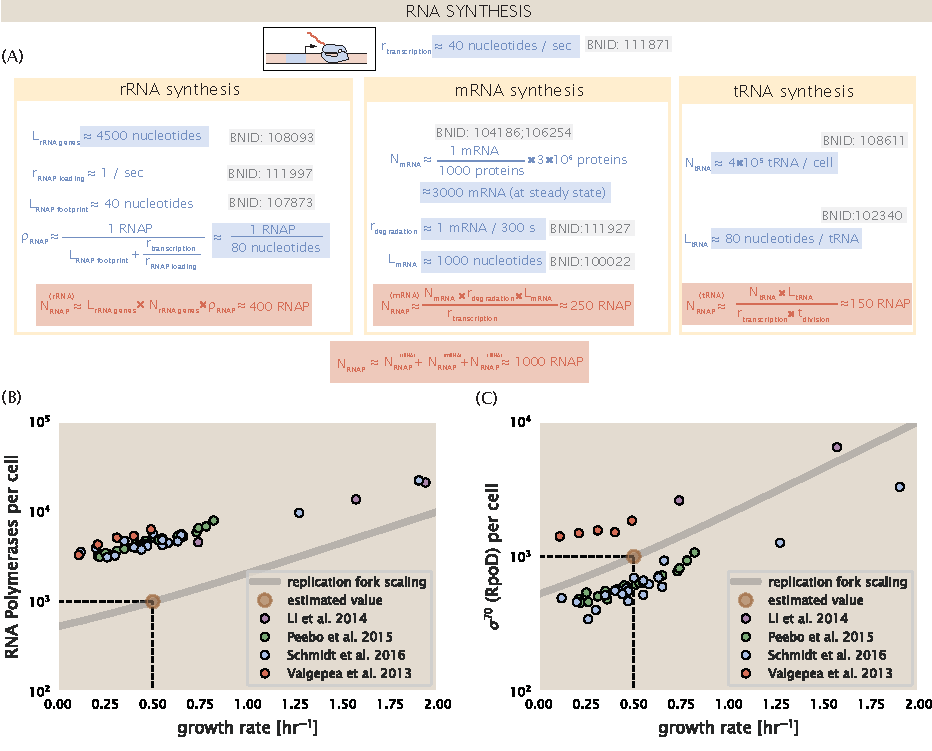
\includegraphics{main_figs/fig7_RNA_synthesis.pdf}
        \caption{\textbf{Estimation of the RNA polymerase demand and
        comparison with experimental data.} (A) Estimations for the number of
        RNA polymerase needed to synthesize sufficient quantities of rRNA, mRNA,
        and tRNA from left to right, respectively.(B) The RNA
        polymerase core enzyme copy number as a function of growth rate. Colored
        points correspond to the average number RNA polymerase core enzymes that
        could be formed given a subunit stoichiometry of [RpoA]$_2$[RpoC][RpoB].
        (C) The abundance of $\sigma^{70}$ as a function of growth rate.
        Estimated value for the number of RNAP is shown in (B) and (C) as a
        translucent brown point at a growth rate of 0.5 hr$^{-1}$.}
    \label{fig:RNA_synthesis}
    }
    \end{fullwidth}
\end{figure}
